Before using the inexact product in big problems, simpler examples are used to validate the approach and fix minor parameters in the scheme.

The two firsts tests evaluate the speedup in the product of a Hierarchical Matrix and a vector and an exection of the Inexact GMRES with few iterations, using the operators obtained through 2nd type Equations of Laplace and Helmholtz \ref{eq:pde_helmlaplace}, where the last one is a scaterring problem, where $\Delta$ is the Laplace operator and everything is suposed to be solved in two dimentions. The last test will use a cavity problem to test the speedup of the algorithm in a situation with more iterations.

\begin{align}\label{eq:pde_helmlaplace}
    \begin{split}
        \Delta u &= 0 \\
        \Delta u + k^{2}u &= 0
    \end{split}
\end{align}

Reformulationg both equations as a Boundary Integral Equation, the simple \textit{direct} formulation is used to write the solution as \ref{eq:direct_formulation}, where $\Gamma$ is boudnary of the domain, \textit{S} and \textit{D} are the single and double layer operators, defined as \ref{eq:single_double}, and $G(x,y)$ is the fundamental solution of the desired PDE.

\begin{equation}\label{eq:direct_formulation}
    -\frac{u(x)}{2} + D[u](x) = S[\partial_{\nu }u] (x), \hspace{0.3in} x \in \Gamma
\end{equation}

\begin{align}\label{eq:single_double}
    \begin{split}
        S[\sigma](x) &= \int_{\Gamma} G(x,y) \sigma(y)  \,ds(y) \\
        D[\sigma](x) &= \int_{\Gamma} \frac{\partial G}{\partial \nu_{y}}(x,y) \sigma(y)  \,ds(y)
    \end{split}
\end{align}

For the first to examples, a unit circle around the origin is used as the boundary to generate the operators, with the mesh being created with the Inti library \cite{git-inti}.

For the last test, the mesh is made from a cavity $.geo$ file avaiable in \cite{git_dudu}. A view of the figure can be seen in \ref{fig:cavity_fig}. The incident wave' angle is chosen to be $\frac{\pi}{4}$ rad.

\begin{figure}[h!]
    \centering
    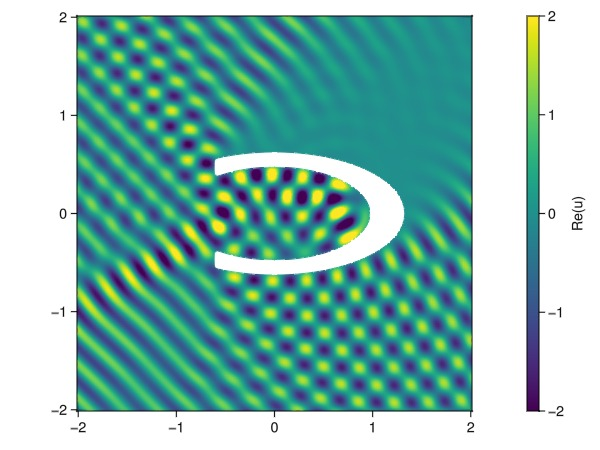
\includegraphics[width=0.6\linewidth]{images/cavity_fig.jpg}
    \caption{Geometry used in the test.}
    \label{fig:cavity_fig}
\end{figure}


\section{Laplace's results}

All results are contained in \ref{fig:laplace_results}, showing the evolution of the residual with the product tolerance aswell as the speedup to each of these values.

\begin{figure}[h!]
    \centering
    \includesvg[width=0.6\linewidth]{images/fixed_size_laplace_product.svg}
    \caption{Speedup and residual evolution for the product between a 8000x8000 HMatrix and a vector.}
    \label{fig:laplace_results}
\end{figure}

\section{Helmholtz's results}


For the unitary circle boundary the results can be seen in \ref{fig:Helmholtz_circle_results}.

\begin{figure}[h!]
    \centering
    \begin{subfigure}[b]{0.45\linewidth}
        \includesvg[width=\linewidth]{images/fixed_size_helmholtz_product.svg}
        \caption{Results for the product of a 70000x 70000 HMatrix and a vector.}
    \end{subfigure}
    \begin{subfigure}[b]{0.45\linewidth}
        \includesvg[width=\linewidth]{images/fixed_size_helmholtz_gmres.svg}
        \caption{Results for an initial application of the Inexact GMRES algorithm.}
    \end{subfigure}
    \caption{Results for the application of the Inexact GMRES algorithm with a 70000x70000 HMatrix.}
    \label{fig:Helmholtz_circle_results}
\end{figure}


For the cavity, \ref{fig:cavity_results}.

\begin{figure}[h!]
    \centering
    \includesvg[width=0.6\linewidth]{images/fixed_size_helmholtz_cavity.svg}
    \caption{Speedup witnessed in the application of the Inexact GMRES in a 50000x50000 matrix.}
    \label{fig:cavity_results}
\end{figure}

An evolution of the number of iterations in face of the different tolerances passed to the algorithm is in \ref{fig:cavity_iterations}.

\begin{figure}[h!]
    \centering
    \includesvg[width=0.6\linewidth]{images/fixed_size_helmholtz_cavity_iterations.svg}
    \caption{Evolution of the quantity of iterations needed for convergence and overall tolerance passed as an argument.}
    \label{fig:cavity_iterations}
\end{figure}